\section{Schraubenverbindungen}
\begin{vardef}
	\item[$P$] Steigung in mm (Höhenunterschied bei einem Umlauf)
	\item[$\alpha$] Windungssteigungswinkel
	\item[$\beta$] Flankenöffnungswinkel (bei metrischen Schrauben $\beta=60\degree$)
	\item[$d_2$] mittlerer Flankendruchmesser
	\item[$d_3$] Kerndurchmesser
	\item[$d$] Nenndruchmesser (Gewindeaußendruchmesser)
	\item[$d_\text{K}$] Kopfdruchmesser (=Schlüsselweite)
	\item[$D_\text{B}$] Bohrungsdurchmesser (Da wo die Schraube rein soll, am besten kleiner als Kopfdurchmesser)
	\item[$r_\text{A}$] Mittlerer belasteter Durchmesser des Schraubenkopfs
	\item[$A_\text{K}$] Schraubenkopfauflagefläche
	\item[$A_\text{S}$] gefährdeter Spannungsquerschnitt der Schraube (tabelliert)
	\item[$\varrho'$] Winkel des Reibungskegels
	\item[$\mu$] Reibungskoeffizient
	\item[$c_\text{s}$] Federrate der Schraube
	\item[$c_\text{p}$] Federrate der Zwischenlage
	\item[$\Phi$] Kraftverhältnis
	\item[$\Phi_\text{n}$] Kraftverhältnis unter Berücksichtigung des Krafteinleitungsfaktor
	\item[$F_\text{KL}$] Klemmkraft (Kraft in der Verbindungsfuge)
	\item[$F_\text{A}$] Axiale Betriebskraft (Kraft, die die verbundenen Teile auseinander zieht; immer Zugkraft!)
	\item[$F_\text{S}$] Schraubenkraft (Kraft in der Schraube, die die Schraube dehnt)
	\item[$F_\text{SA}$] Schraubenzusatzkraft	\item[$F_\text{PA}$] Kraft der Zwischenlage
	\item[$F_\text{VM}$] Montagevorspannkraft
	\item[$F_\text{z}$] Vorspannkraftverlust durch Setzerscheinung
	\item[$f_\text{z}$] Setzbetrag
	\item[$M_\text{G}$] Moment am Gewinde
	\item[$M_\text{K}$] Moment am Kopf
	\item[$M_\text{A}$] Anziehmoment
	\item[$n$] Krafteinleitungsfaktor
	\item[$\alpha_\text{A}$] Anziehfaktor (Unschärfe bei der Montage der Schraube)
\end{vardef}

% Windungssteigungswinkel
\hrule
\begin{eeqn}{Windungs\-steigungs\-winkel}
	\begin{align}
	\alpha &= \arctan{\left(\frac{P}{\pi \cdot d_2}\right)}
	\end{align}
\end{eeqn}

% Reibungswinkel
\begin{eeqn}{Reibungs\-winkel}
	\begin{align}
	\varrho' &= \arctan{\left(\frac{\mu}{\cos{\left(\frac{\beta}{2}\right)}}\right)}
	\end{align}
\end{eeqn}

% Kraftverhältnis
\begin{eeqn}{Kraftverhältnis}
	\begin{align}
		\Phi & = \frac{c_\text{s}}{c_\text{s}+c_\text{p}}
	\end{align}
	Wenn die Krafteinleitungstiefe berücksichtigt wird (immer im Zusammenhang mit $F_\text{A}$)
	\begin{align}
		\Phi_\text{n} & = \frac{c_\text{s}}{c_\text{s}+c_\text{p}} \cdot n
	\end{align}
\end{eeqn}

% Kopfgeometrie
\begin{eeqn}{Geometrie des Schraubenkopfs}
	\begin{align}
		& r_\text{A} = \frac{d_\text{K}+D_\text{B}}{4} \\
		& A_\text{K} = \frac{\pi}{4} \cdot (d_\text{k}^2-D_\text{B}^2)
	\end{align}
	Es muss auf eventuelle Fasen an der Bohrung geachtet werden, der Bohrungsdurchmesser $D_\text{B}$ vergrößert sich entsprechend.
\end{eeqn}

% Wirkungsgrad
\begin{eeqn}{Wirkungsgrad}
	\begin{align}
		\eta & = \frac{\tan \alpha}{\tan(\alpha + \varrho')}
	\end{align}
\end{eeqn}

% Setzkraftverlust in der Schraube
\begin{eeqn}{Setzkraftverlust}
	\begin{align}
		& F_\text{Z} = f_\text{z} \cdot c_\text{p} \cdot \Phi
	\end{align}
	Durch Mikroplastizitäten in den Kontaktflächen der Verbindung findet eine Entlastung der selbigen statt. 
\end{eeqn}

% Montagevorspannkraft
\begin{eeqn}{Montagevorspannkraft}
	\begin{align}
		& F_\text{VM,min} = F_\text{KL} + F_\text{A}\cdot (1-\Phi_\text{n})+F_\text{Z} \\
		& F_\text{VM} = \alpha_\text{A}\cdot F_\text{VM,min}
	\end{align}
\end{eeqn}

% Moment zum Lösen der Schraube
\begin{eeqn}{Moment zum Lösen der Schraube}
	\begin{align}
		& F_\text{S} = F_\text{KL} + F_\text{A}\cdot (1-\Phi_\text{n}) \\
		& M_\text{Lös} = F_\text{s} \cdot \tan (\alpha - \varrho') \cdot \frac{d_2}{2}
	\end{align}
	Moment am Gewinde ohne den Anteil des Setzbetrags
\end{eeqn}

% Moment am Kopf
\begin{eeqn}{Moment am Kopf}
	\begin{align}
		M_\text{K} & = F_\text{VM} \cdot \mu \cdot r_\text{A}
	\end{align}
\end{eeqn}

% Moment am Gewinde
\begin{eeqn}{Moment am Gewinde}
	\begin{align}
		& M_\text{G} = F_\text{VM} \cdot \frac{d_2}{2} \cdot \tan{(\alpha+\varrho')}
	\end{align}
\end{eeqn}

% Anziehmoment
\begin{eeqn}{Anziehmoment}
	\begin{align}
		& M_\text{A} = M_\text{K} + M_\text{G}
	\end{align}
\end{eeqn}


% Pressung am Kopf der Schraube
\begin{eeqn}{Pressung am Kopf der Schraube}
	\begin{align}
		P &= \frac{F_\text{VM}+F_\text{A}\cdot\Phi_\text{n}}{A_\text{K}}
	\end{align}
\end{eeqn}

\newpage

Um die Federrate einer Schraube zu berechnen muss man sie zerlegen. Das geschieht je nach Schraubenart wie unten dargestellt:
\begin{figure}[h]
\centering
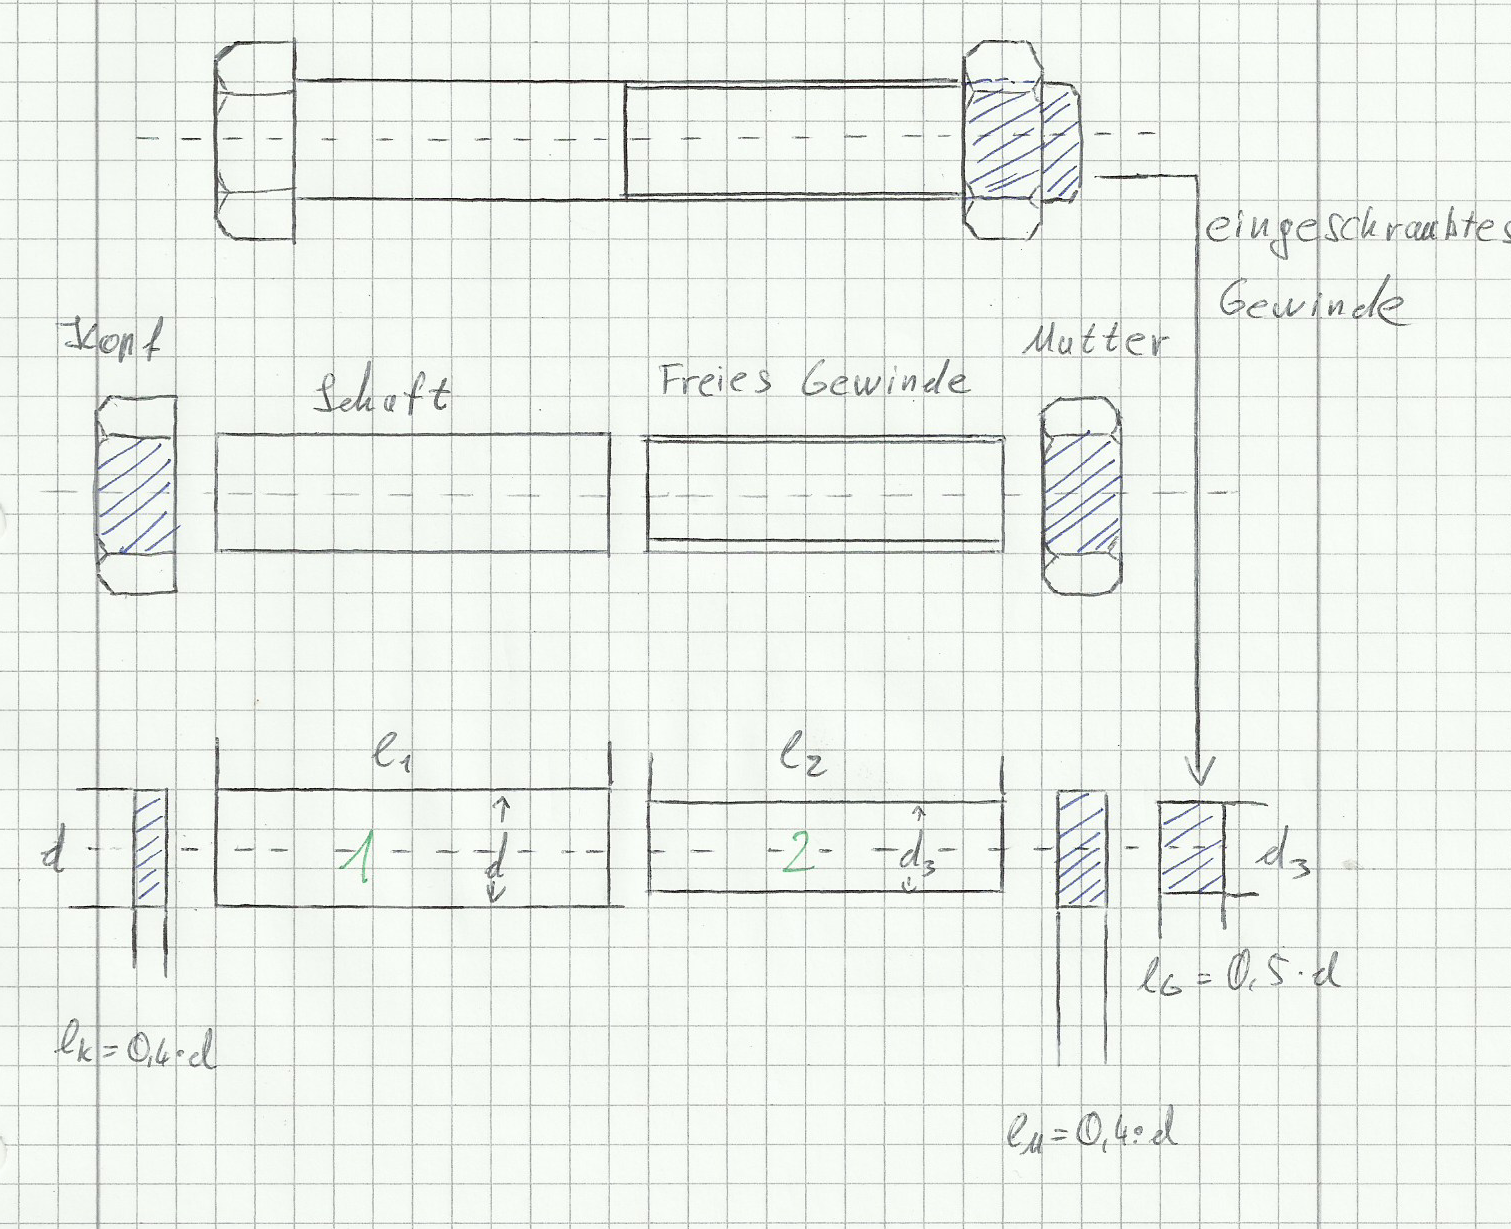
\includegraphics[scale=0.5]{schrauben/Federrate_Schrauben_1.png}
\caption{Normalschaftschraube}
\end{figure}

Die Berechnung erfolgt dann zuerst pro Zylinder so:

\begin{align*}
C &= \frac{E \cdot A}{l} \qquad \text{mit} \qquad A = \frac{\pi}{4} \cdot D^2
\intertext{Im oben dargestellten Fall würde sich die Gesamtfederrate so ergeben:}
\frac{1}{C_{ges}} &= \frac{1}{C_1} + \frac{1}{C_2} + \frac{1}{C_K} + \frac{1}{C_M} + \frac{1}{C_G} \\
\Leftrightarrow C_{ges} &= \frac{1}{\frac{1}{C_1} + \frac{1}{C_2} + \frac{1}{C_K} + \frac{1}{C_M} + \frac{1}{C_G}}
\end{align*}


\newpage

\begin{figure}[h]
\centering
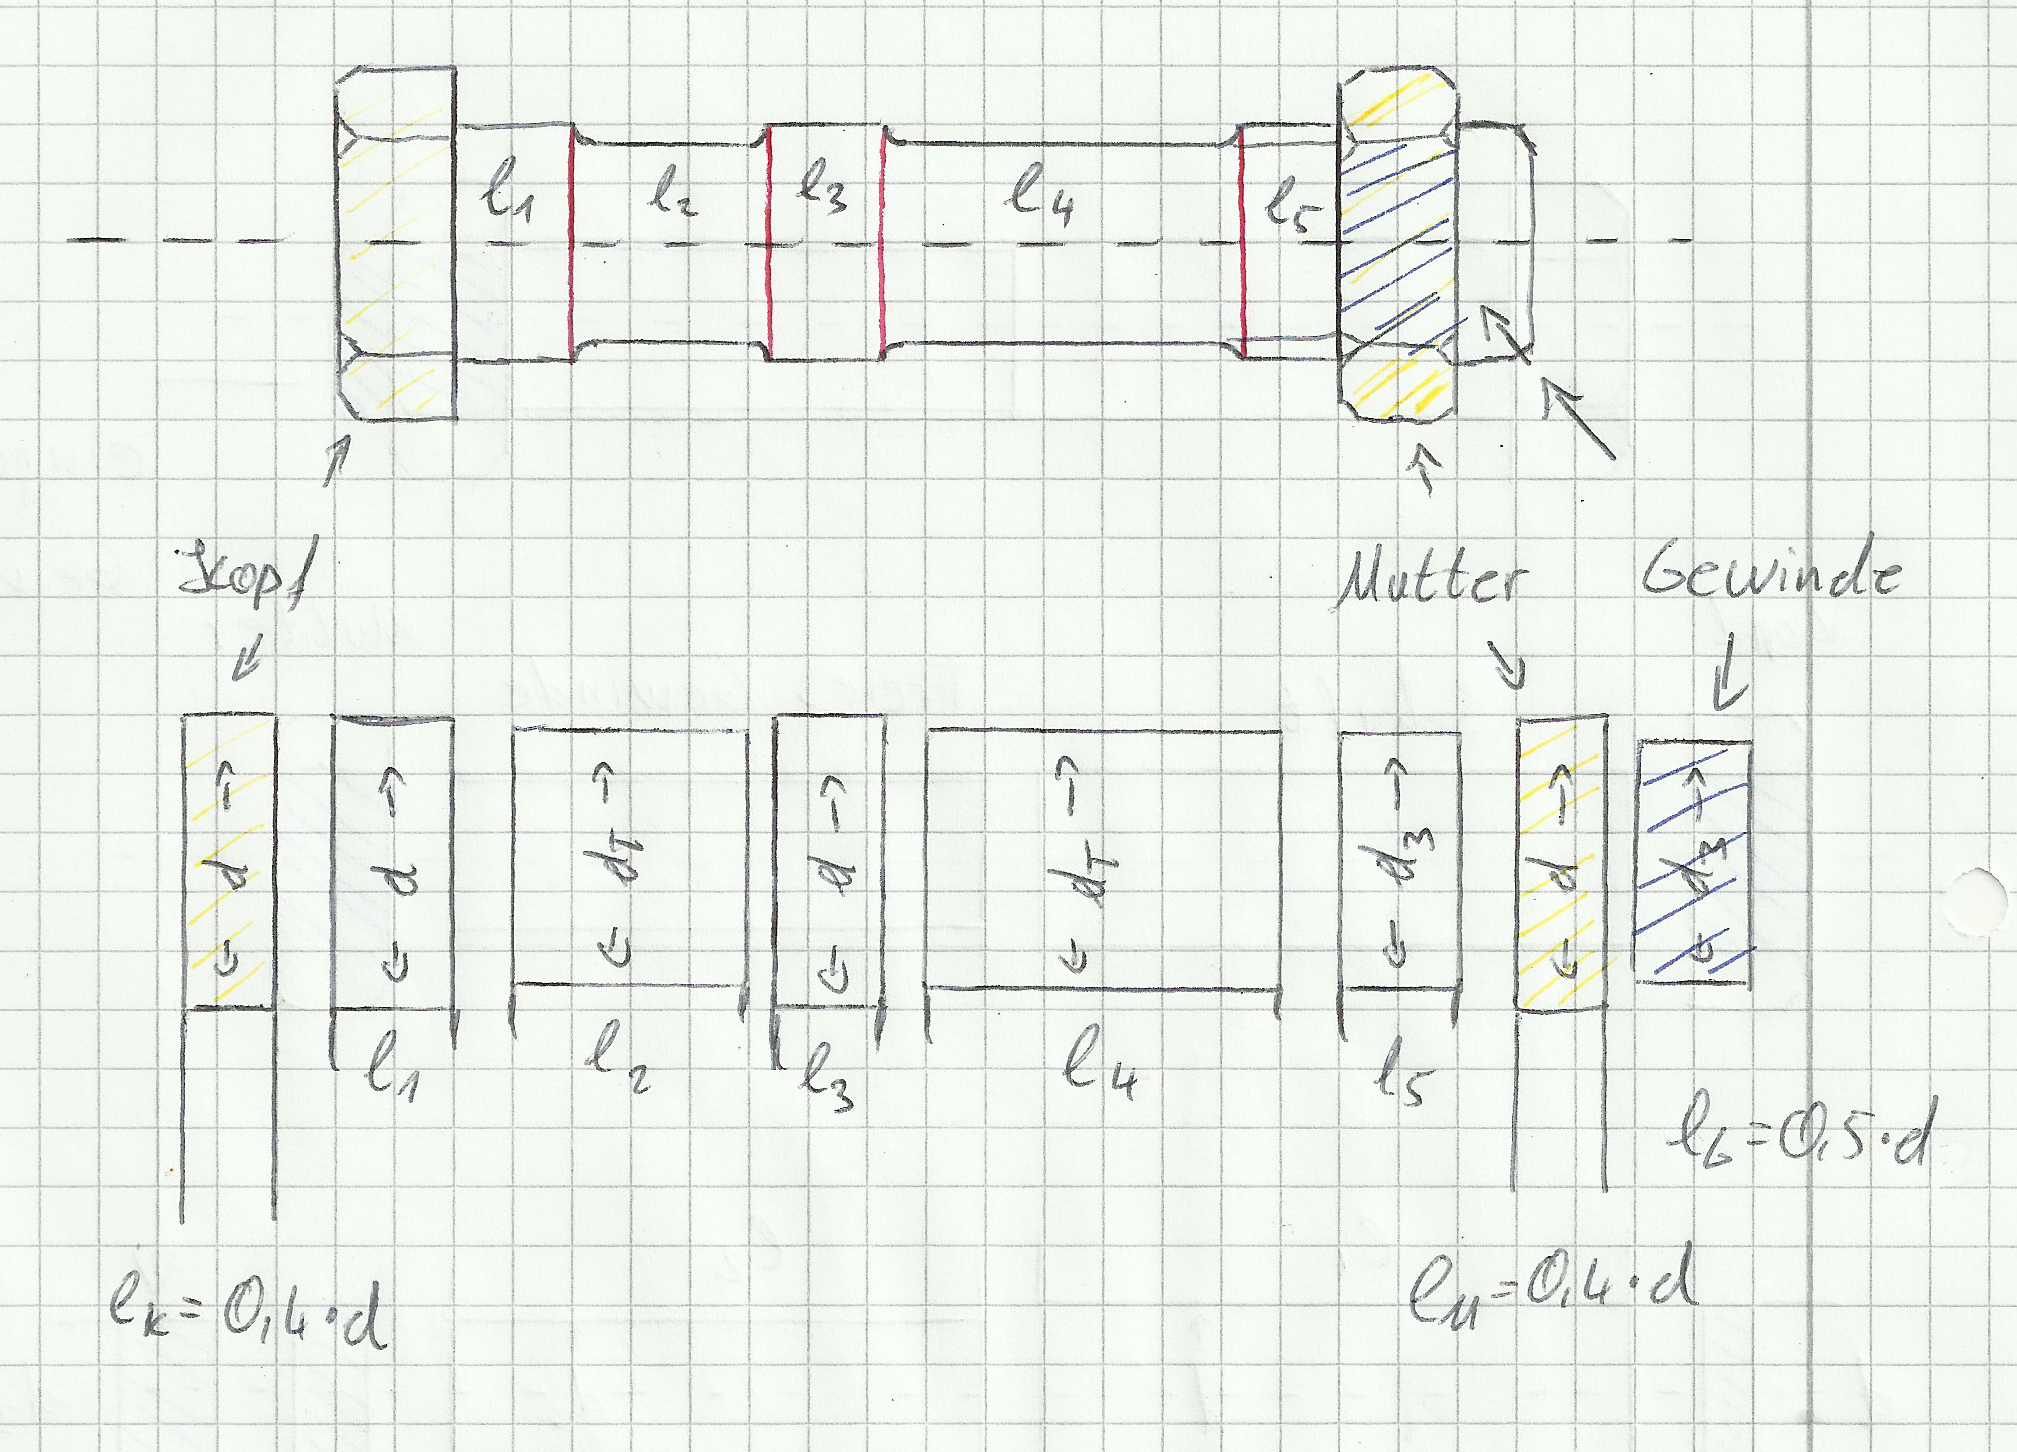
\includegraphics[scale=0.45]{schrauben/Federrate_Schrauben_2.png}
\caption{Dünnschaftschraube}
\end{figure}


Die Berechnung erfolgt dann zuerst pro Zylinder so:

\begin{align*}
C &= \frac{E \cdot A}{l} \qquad \text{mit} \qquad A = \frac{\pi}{4} \cdot D^2
\intertext{Im oben dargestellten Fall würde sich die Gesamtfederrate so ergeben:}
\frac{1}{C_{ges}} &= \frac{1}{C_1} + \frac{1}{C_2} + \frac{1}{C_3} + \frac{1}{C_4} + \frac{1}{C_5} + \frac{1}{C_K} + \frac{1}{C_M} + \frac{1}{C_G} \\
\Leftrightarrow C_{ges} &= \frac{1}{\frac{1}{C_1} + \frac{1}{C_2} + \frac{1}{C_3} + \frac{1}{C_4} + \frac{1}{C_5} + \frac{1}{C_K} + \frac{1}{C_M} + \frac{1}{C_G}}
\end{align*}

\newpage

\hrule
% Spannugen in der Schraube
\begin{eeqn}{Spannungen in der Schraube}
	\begin{align}
		\sigma_\text{v} &= \sqrt{\left(\frac{F_\text{VM}+F_\text{SA}}{A_\text{S}}\right)^2+3\cdot \left(\frac{16 \cdot M_\text{G}}{\pi \cdot d_3^3}\right)^2} \label{eqn:spannungen_schraube}
	\end{align}
	Es gilt $F_\text{SA} = F_\text{A}\cdot \Phi_\text{n}$. Die erhaltenen Vergleichsspannung muss kleiner sein als die Streckgrenze $R_\text{e}$ der Schraube. Diese ergibt sich aus den Festigkeitsangaben der Schraube bzw. Mutter. Die Bezeichnung lautet immer $x.y$ wobei $x=R_\text{m}/100$ und $y=R_\text{e}/R_\text{m}$ (es ist immer $y < 1$). Es gilt:
	\begin{align}
		R_\text{e} &= x \cdot 100 \cdot y ~\text{N/mm}^2
	\end{align}
\end{eeqn}


% dynamisch belastete Schrauben
\begin{eeqn}{dynamisch belastete Schrauben}
	\begin{enumerate}[itemsep=0mm,leftmargin=12pt]
	\item Berechnung der Schraubenzusatzkräfte für beide Amplituden ($F_\text{SA,1}$, $F_\text{SA,1}$):
	\begin{align}
		F_\text{SA} &= F_\text{A}\cdot \Phi_\text{n}
	\end{align}
	\item Berechnung der Mittelspannung $\sigma_\text{v}$ mit der größeren Schraubenzusatzkraft gemäß Formel \ref{eqn:spannungen_schraube}.
	\item Ermitteln der mittlere Schraubenzusatzkraft $F_\text{SA,m}$:
	\begin{align}
		F_\text{SA,m} &= \frac{F_\text{SA,1} + F_\text{SA,2}}{2}
	\end{align}
	Diese ergibt mit dem Spannungsquerschnitt die Ausschlagsspannung $\sigma_\text{a}$:
	\begin{align}
		\sigma_\text{a} &= \frac{F_\text{SA,m}}{A_\text{S}}
	\end{align}
	\item Im Betriebszustand pendelt die Spannung um $\pm \sigma_\text{a}$ und hat die Mittelspannung $\sigma_{v}$.
	\end{enumerate}
	Umso kleiner $\Phi_\text{n}$ ist, desto besser ist die Schraubverbindung für dynamische Belastungen geeignet (Die Ausschlagsspannugen sind kleiner bei kleinem $\Phi_\text{n}$).
	Es gilt die Römerformel $\sigma_\text{a} \le 0,07 \cdot R_\text{E}$, ist diese Bedingung nicht erfüllt, müssen entweder mehr Schrauben verwendet werden oder der Faktor $\Phi_\text{n}$ verkleinert werden. \\
\end{eeqn}

\begin{figure}[H]
	\centering
	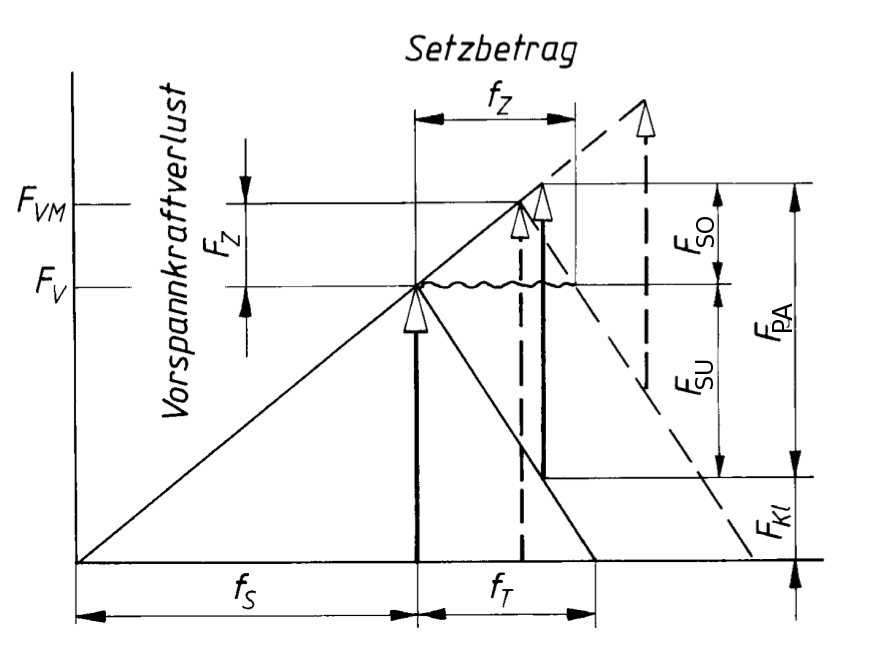
\includegraphics[width=0.8\linewidth]{schrauben/schraubendiagramm}
	\caption*{Schraubendiagramm einer dynamisch belasteten Schraube mit Setzerscheinung}
\end{figure}


% Auslegung von Schrauben
\hrule
\begin{eeqn}{Auslegung von Schrauben}
	\begin{enumerate}[itemsep=0mm,leftmargin=12pt]
		\item Wahl der Festigkeitsklasse (wenn nicht anders angegeben: 8.8 / $R_\text{e}=\SI{640}{N/mm^2}$) und errechnen von $R_\text{e}$.
		\item Ermittlung der zulässigen Spannung gemäß der Römerformel ($\mu_\text{Stahl}=0,15$):
			\begin{align}
				\sigma_\text{zul} &= (0,85-\mu)\cdot R_\text{e}
			\end{align}
		\item Bestimmung des Spannungsquerschnitts bei gegebener Schraubenkraft $F_\text{S}=F_\text{KL}+F_\text{A}$ (Beim Auslegen gilt, wenn nichts anderes angegeben: $F_\text{A}=0$; $\alpha_\text{A}=1$):
			\begin{align}
				A_\text{S} &\geq \frac{\alpha_\text{A} \cdot F_\text{S}}{\sigma_\text{zul}}
			\end{align}
		\item Aus Tabellen kann mit dem gefundenen Spannungsquerschnnitt eine Schraube ausgewählt werden. Mit der gewählten Schraube sollten Pressung und Spannungen überschlagsmäßig überprüft werden, hierfür muss zunächst die Schraubenauflagefläche $A_\text{K}$ berechnet werden.
	\end{enumerate}
\end{eeqn}